\documentclass[a4paper,10pt]{report}
\usepackage[T1]{fontenc}
\usepackage[table]{xcolor}
\usepackage{titlesec}
\usepackage{graphicx}
\usepackage[inkscapepath=../assets/svg]{svg}
\usepackage{amsmath}
\usepackage{amsthm}
\usepackage{mathtools}
\usepackage{fancyvrb}
\usepackage[english]{babel}
\usepackage{csquotes}
\usepackage{hyperref}
\hypersetup{
   colorlinks=true,
   linkcolor=blue,
   urlcolor=cyan
}
\usepackage{tikz}
\usepackage{amssymb}
\usepackage[sc]{mathpazo}
\linespread{1.05}
\usepackage{microtype}
\usepackage{breqn}
\usepackage{caption}
\usepackage{subcaption}
\usepackage[
   backend=bibtex,%
   bibencoding=utf8,%
   language=english,%
   style=numeric-comp,%
   sorting=nyt,%
   maxbibnames=10,%
   natbib=true%
]{biblatex}
\addbibresource{references.bib}
\usepackage{siunitx}
\usepackage{booktabs}
\usepackage{longtable}
\usepackage{geometry}
\usepackage{multirow}
\graphicspath{ {../assets/img/} }

\newgeometry{hmargin={30mm,30mm}}

% Set TOC depth and sections numbering
\setcounter{tocdepth}{3}
\setcounter{secnumdepth}{3}

% Remove chapters head and reduce spacing
\titleformat{\chapter}[hang]{\Large\bfseries}{\thechapter \hspace{2ex}}{0pt}{\Large}
\titlespacing{\chapter}{0cm}{0cm}{0.5cm}
\usepackage[parfill]{parskip}

% Make quotes italic
\renewcommand{\mkbegdispquote}[2]{\itshape}

% Change texttt line breaks
\renewcommand{\texttt}[1]{%
  \begingroup
  \ttfamily
  \begingroup\lccode`~=`.\lowercase{\endgroup\def~}{.\discretionary{}{}{}}%
  \catcode`/=\active\catcode`[=\active\catcode`.=\active
  \scantokens{#1\noexpand}%
  \endgroup
}


\begin{document}
\frenchspacing

% First page
\title{
  {{\large{\textsc{Alma Mater Studiorum $\cdot$ University of Bologna}}}}
  \rule{\textwidth}{0.4pt}\vspace{3mm}
  \textbf{SKA Data Challenge\footnote{The code for the project is publicly available on \href{https://github.com/Lorenz92/SKADC1}{GitHub}}}
  \begin{figure}[!htb]
    \centering
    
\includegraphics[width = 100pt]{squad-logo}
  \end{figure} \\
  Deep Learning course final project
}

\author{Alice Zandegiacomo (\href{mailto:alice.zandegiacomo@studio.unibo.it}{alice.zandegiacomo@studio.unibo.it}) \\ Lorenzo Cellini (\href{mailto:lorenzo.cellini3@studio.unibo.it}{lorenzo.cellini3@studio.unibo.it})}
\date{\today}
\maketitle
\newpage
\tableofcontents
\setcounter{tocdepth}{1}
%\listoffigures
%\listoftables
\newpage


\chapter{Summary}\label{chap:introduction}

The tasks of object detection and classification have gained significant popularity over the past years within the deep learning and computer vision communities. Systems trained end-to-end now achieve great results on a variety of tasks in the video and image domains.

In this work, we address an object detection and classification problem on the Square Kilometer Array Dataset (SKADC1) \cite{ska-site}: given a large image, of about 32,000 pixels on each side and 4GB in size, the goal is to detect astronomycal sources and classify them among three possible classes.

This project focuses on the SKADC1 dataset, in particular on the 560MHz-1000h high S/N sky image, that contains more than \num{19000} radio sources.

Among the state of the art types of network, we opted for a two-stage system, specifically a Faster R-CNN.

In this work we implemented and compared three different models:
\begin{enumerate}
  \item B16: a Faster R-CNN with a naive feature extraction backbone with only 4 convolutional layers and with a receptive field of 16 on the last convolutional layer, that will act as our baseline model;
  \item B44: a Faster R-CNN with a feature extraction backbone with 7 convolutional layers and a receptive field of 44 on the last convolutional layer;
  \item A Faster R-CNN with a larger backbone, specifically we implemented a VGG16 backbone, COMPLETAQUI \cite{bidaf}
\end{enumerate}
Each model consists of the same input and output (Region Proposal Network + Detector) structure, and what changes is the deepness of the feature extraction network (usually called backbone).

In training the listed models, we adopted a transfer learning technique, because it has been proven to be effective in speeding up the training phase. 
More specifically, we applied transfer learning only on the very first layers in order to inherit and retain the more basic feature, while letting the model learn deeper representation of them.

So each model is initialized with the VGG16 public weights, then we freezed the first four convolutional layers and let deeper ones trainable.

While this could seem an easy object detecion and classification problem, it turns out that it is an hard task on both the goals:
\begin{itemize}
  \item the objects to be located are very small, as we will show later, and
  \item the dataset is extremely unbalanced with respect to class distribution.
\end{itemize}

For this two reasons we developed more than one model and we made some choices that will be discussed later.

Our experimental evaluations show that the best model is  ... Such results are on par with those reported in the corresponding models' papers.

\chapter{Background}\label{chap:background}

-- QUI DARE LE DEFINIZIONI DI YOLO SSD E FASTER RCNN + DESCRIZIONE DETTAGLIATA DEI MODULI DI FASTER RCNN --

As already described above, the question answering task is based on the idea of identifying one possible answer to the given question as a subset of the given context.

Since the input data is of textual form and the latest models for the task are all based on neural architectures, there is the need to encode such text into a numeric representation. As of today, there are two main approaches to embed words in numerical format: sparse embeddings, like TF-IDF \cite{tf-idf} and PPMI \cite{ppmi}, and the modern dense embeddings, such as Word2Vec \cite{word2vec} and GloVe \cite{glove}. In the latter case, embeddings for each word in the input vocabulary are usually computed with shallow encoders.

These embeddings are then used as inputs for models specialized in processing sequences. Nowadays, such models are mostly based on the Transformer architecture \cite{transformers}, which has the attention mechanism at its core. Instead, before this revolution, NLP competition's leaderboards were mostly populated by models based on recurrent and convolutional modules.

The most influential recurrent networks are LSTMs \cite{lstm} and GRUs \cite{gru}. They are both based on processing sequential inputs and they keep an evolving series of hidden states, such that the output $h_t^{(0)}$ is a function of $h_{t-1}^{(0)}$ and the input $x_t$ at position $t$. Recurrent layers can also be stacked to increase the capacity of the network: in that case, $h_t^{(0)}$ would act as an input to $h_t^{(1)}$, i.e. the first hidden state of the next depth-wise layer, and the same goes for the successive layers, as shown in figure \ref{fig:recurrent}.

\begin{figure}[h]
  \center
  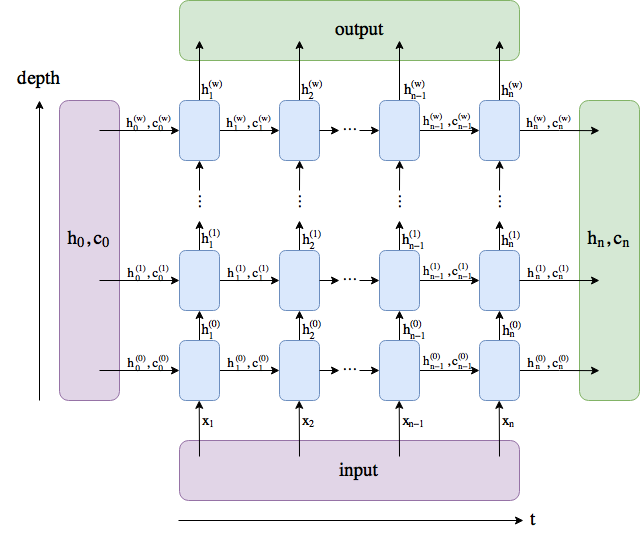
\includegraphics[width=0.65\linewidth]{recurrent}
  \caption{Recurrent module (image courtesy of \cite{recurrent-img})}
  \label{fig:recurrent}
\end{figure}

In natural language, meaning does not usually simply flow from left to right, so that in RNNs other techniques may be necessary to reach a higher level of understanding. One example of such improvement is bi-directionality: the input is processed in two ways, from left to right (the "forward" pass) and from right to left (the "backward" pass); then, outputs of the two computations are merged together (usually by concatenating them over their last dimension). The intuition behind bi-directional RNNs is that they tend to understand the overall context better than their uni-directional counterparts, since they are able to aggregate information from the "past" and from the "future".

About Transformers, at a high-level, they comprise a stack of encoder-decoder modules, where each encoder features a multi-head attention block (to focus on different subsets of the input sequence when encoding one specific token) and a point-wise fully-connected layer, while each decoder features the same architecture as the encoder, but with an additional multi-head attention block in the middle (that helps the decoder focus on relevant parts of the input sequence).

The multi-head attention modules in the Transformer architecture are the ones responsible for gathering information from other tokens in the input sequence, thus resembling the task of hidden states in RNNs (i.e. incorporate the representation of previous inputs with the currently processed one).

\begin{figure}[h]
  \center
  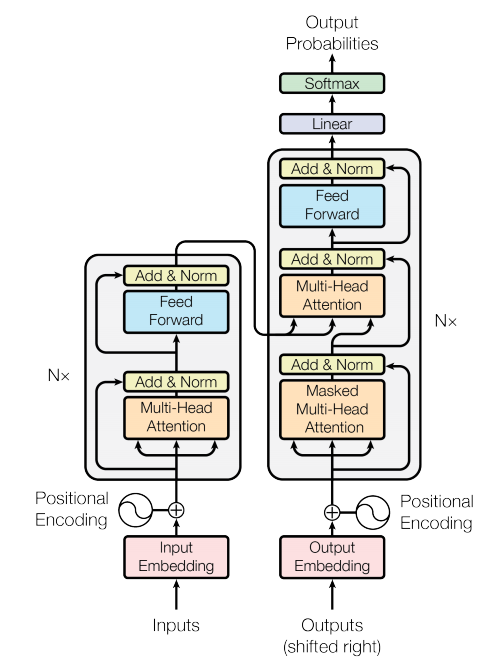
\includegraphics[width=0.45\linewidth]{transformers}
  \caption{Transformers (image taken from \cite{transformers})}
  \label{fig:transformers}
\end{figure}

While Transformers may always seem the way to go, since they throw away all the computational burden of training recurrent modules (which are sequential in nature and, thus, scarcely parallelizable), they also suffer from limitations due to the quadratic complexity of attention and the inherent maximum number of input tokens (which is implicitly linked to architecture choices themselves).

\chapter{Dataset description}\label{chap:dataset-description}

-- qui dire anche che le immagini vengono genrate on the fly e quindi anche l'augmentation, se accesa, viene fatta otf
\chapter{System description}\label{chap:system-description}

In this work, we implemented three different models. All of them are a Faster R-CNN network, but they differ on the backbone and hyperparameters.

In order to perform an effective comparison, the models share the same output architecture.

The following is a detailed description of the models. Beware that in each model section we report everything but what happens in the output module, which is described once in \ref{sec:output-module}.

\section{Feature Extraction Backbone}\label{sec:feature-extraction-backbone}
-- aggiungere citazioni ovunque
\subsection{B16 - Baseline 16}\label{subsec:b16}

The first backbone we implemented has the following structure:
\begin{enumerate}
  \item Block 1: consists of 2 convolutional layers with 3x3x64 filters, followed by a ReLU activation layer and a 2x2 MaxPooling layer with stride 2;
  \item Block 2: consists of 2 convolutional layers with 3x3x128 filters, followed by a ReLU activation layer and a 2x2 MaxPooling layer with stride 2;
\end{enumerate}
Both the blocks have been initialized with the public available VGG-16 weights and \textbf{freezed}.

It has been shown that, in computer vision tasks, the very first layers of a convolutional pipeline, learn the most basic features, as strokes or circles.
So, given that the objects we have to detect have simple shapes, like circles or ellipses, and that we think these kind of basic feature are common across different domains, 
we tried to transfer learning from the VGG-16 and freezing the first layers, the ones that learn most basic features.

As mentioned before, the goal was to detect very small objects, with respect to the dimensions usually detected in other deep learning works.
So we decided to crop the original 32kx32k pixels image into 20x20 pixels patches and rescale them to 100x100 pixels, before feeding the network.
This resemble to zoom-in the image, so that the objects to detect become 5 times bigger.

As we've seen before, the bounding box shapes distribution shows that the 99\% of the objects to detect is smaller than 18x18 pixels and the 90\% is smaller then 8x8 pixels, before rescaling.
After rescaling these values become: 99\% smaller than 90x90 pixels and 90\% smaller then 40x40 pixels.

So, with the B16 model, we wanted to test how a backbone with a receptive field smaller than the objects to detect performs on this task.
Indeed the receptive field of B16 backbone (the feature extraction part) is 16, with a stride of 4. So, given an input image of size 100x100px, the last layer feature maps have a size of 25x25.

In this model we used the follwing values for anchor sizes and ratios:
\begin{itemize}
  \item anchor size: [4, 8, 16, 24, 32, 64]
  \item anchor ratio: [2: 1, 1: 2, 1:1]
\end{itemize}

\subsection{B44 - Baseline 44}\label{subsec:b44}


\begin{figure}[h]
  \center
  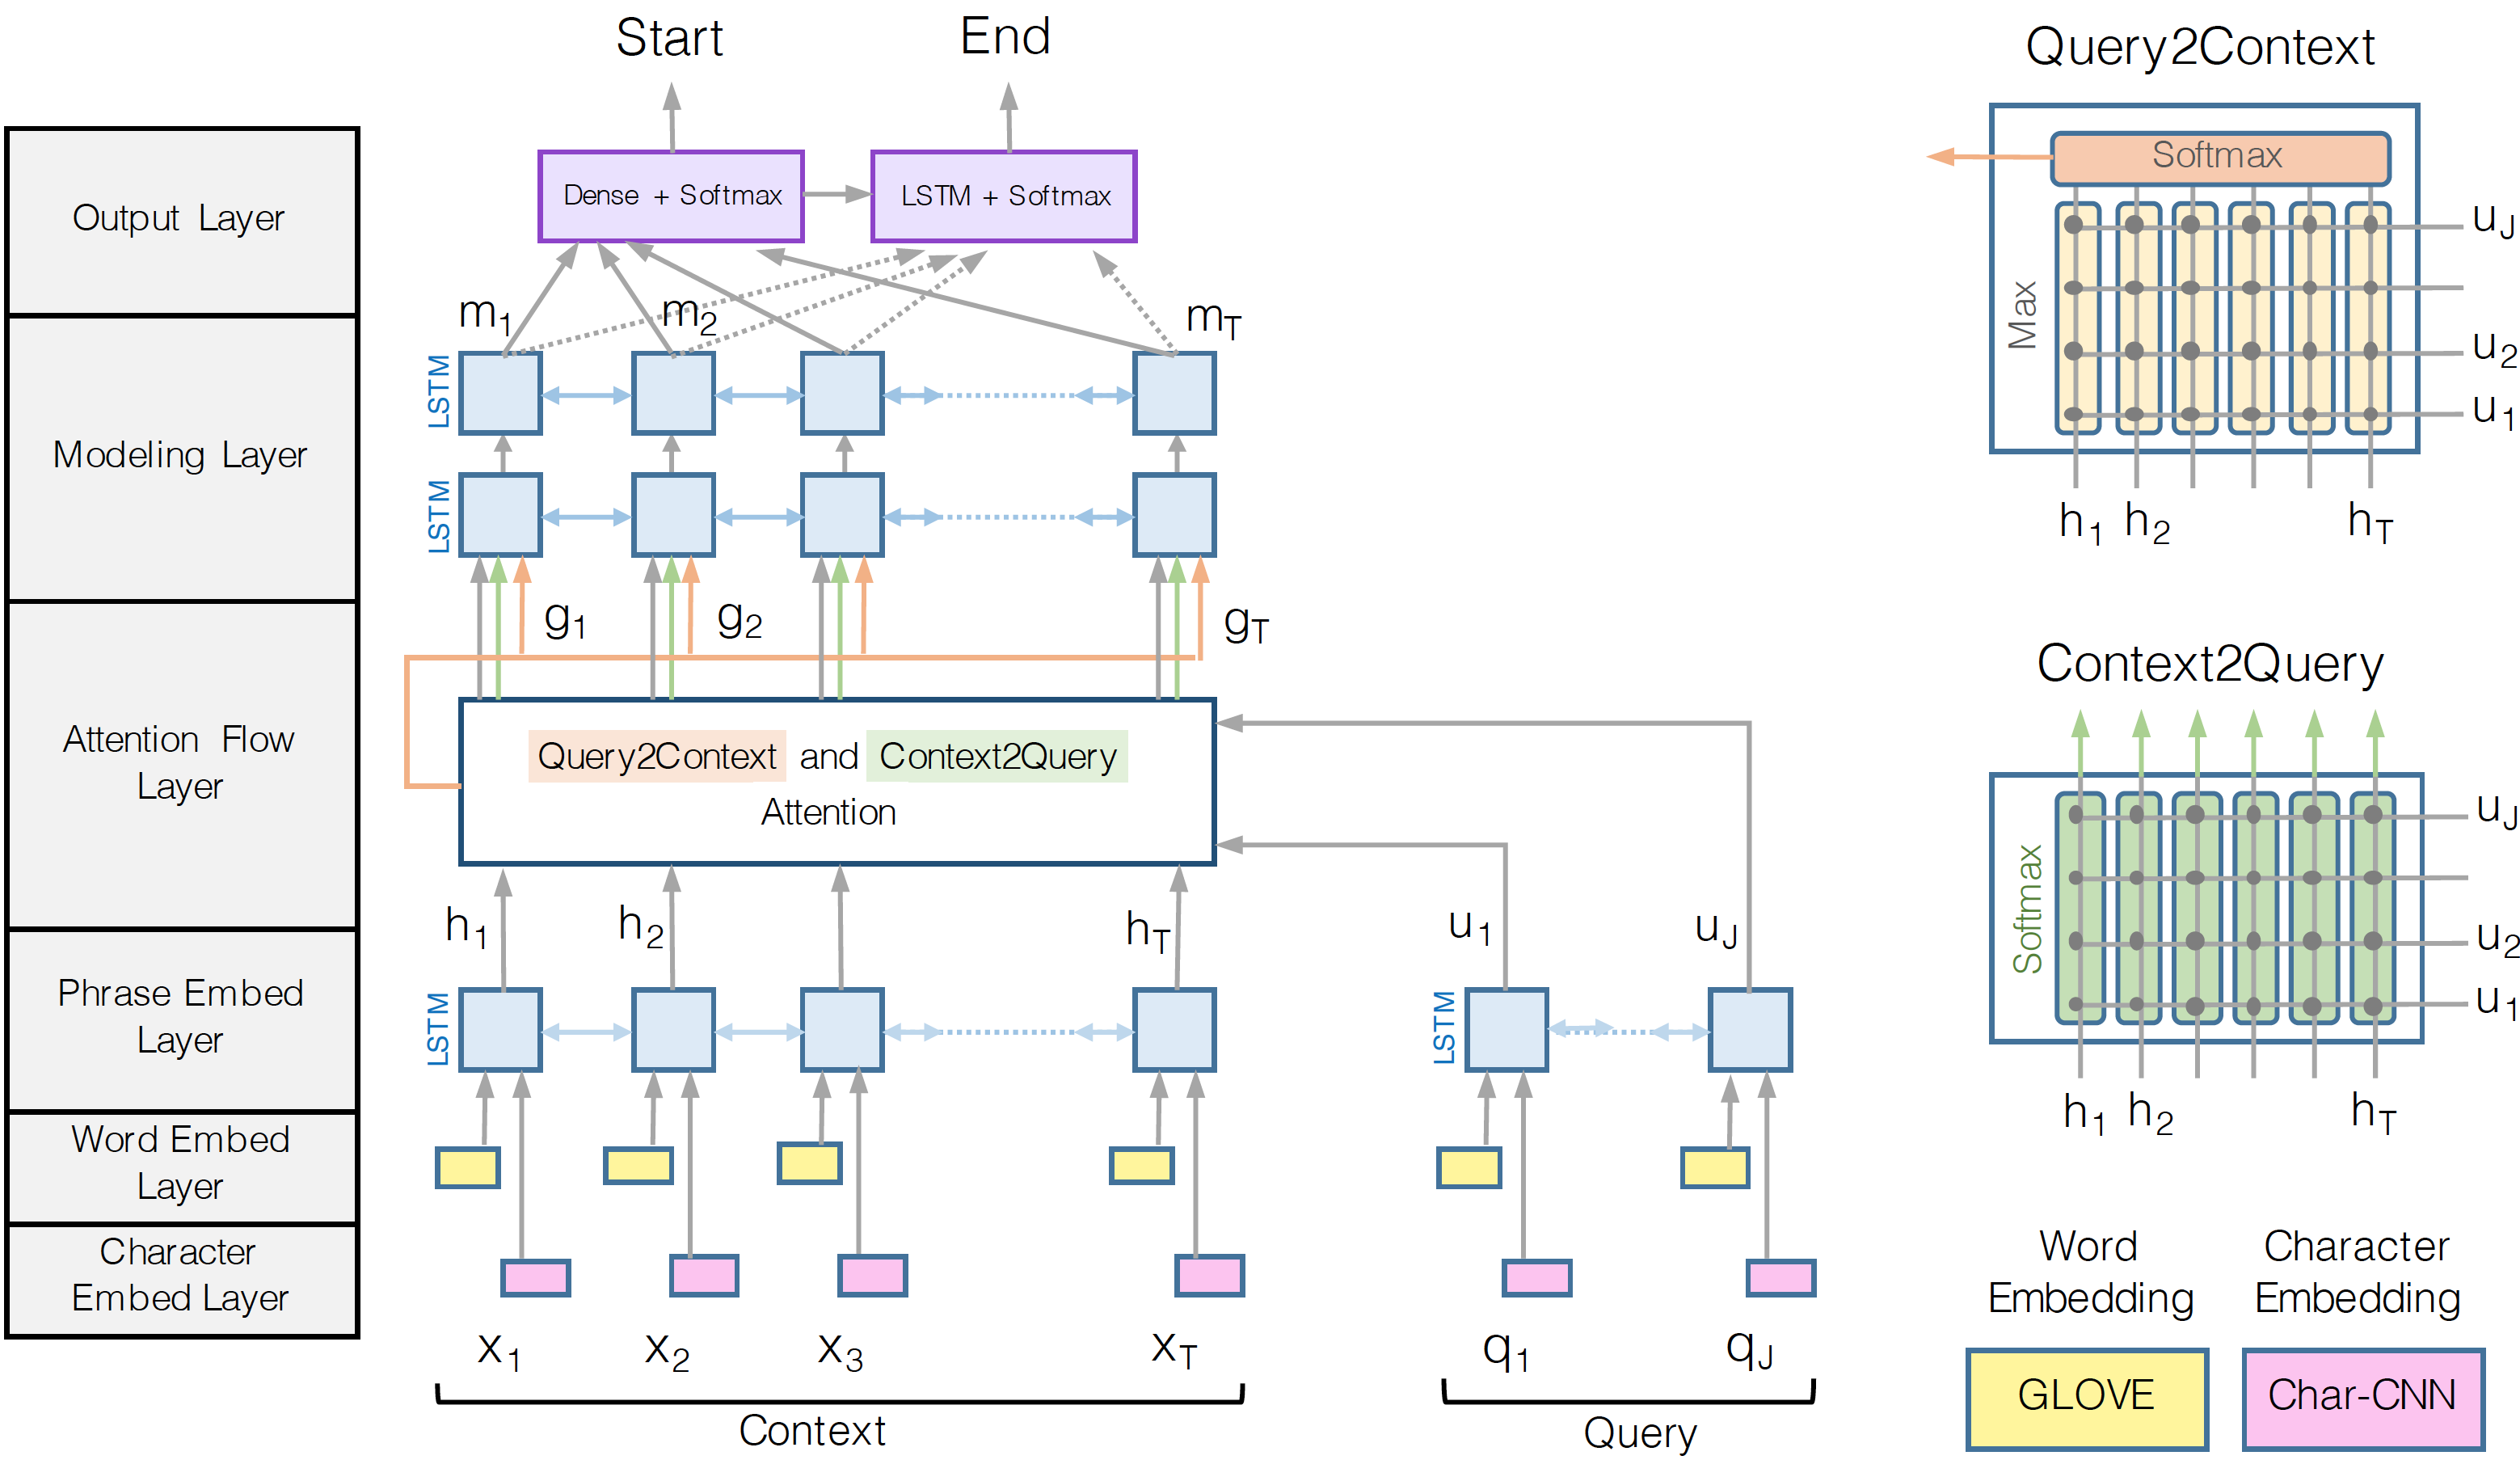
\includegraphics[width=0.85\linewidth]{bidaf}
  \caption{BiDAF model (image courtesy of \cite{bidaf})}
  \label{fig:bidaf}
\end{figure}

\section{Transformer-based models}\label{sec:transformer-models}
\subsection{BERT}\label{subsec:bert-model}
All the Transformer models are based on BERT \cite{bert}, which is a language model composed by a multi-layer bidirectional encoder-decoder structure \cite{transformers}. Our experiments are all performed using the base, uncased implementation of BERT, which has $12$ Transformer layers and $768$ as its hidden size.

The peculiarity of its Transformer architecture allows the model to learn the context of a word based on all of its surroundings, at the same time, without having to perform a sequential scan of the input, as done in standard RNNs. This is reflected in its pre-training, which is composed of two tasks:
\begin{itemize}
  \item Masked Language Modeling (MLM): at a high level, it is performed by masking $15\%$ of the words in each sequence and replacing them with a $[MASK]$ token, so that the model is required to predict the original value of the masked words, using the available ones
  \item Next Sentence Prediction (NSP): achieved giving as input to the model a pair of sentences (formatted as in \ref{sec:tokenization}), which are in $50\%$ of the cases two subsequent sentences or a random picked pair otherwise, so that the model is asked to identify if the second sentence follows the first one in the pair
\end{itemize}
The first task, MLM, is used to gain a detailed understanding of the processed language, while the second task, NSP, is used to let the model have a broader comprehension of semantic connections.

BERT is trained using both tasks together, with the goal of minimizing the combined loss.

\subsection{DistilBERT}\label{subsec:distilbert-model}
BERT performances, as for the majority of large-scale language models, are inevitably intertwined with their number of parameters. DistilBERT \cite{distilbert,distilbert-article} tries to reduce this number using a technique called distillation, which consists in training a smaller "student" network to mimic the full output of the big "teacher" model \cite{distillation}. Specifically, DistilBERT has about half the parameters of BERT and retains $95\%$ of its performance on the GLUE benchmark \cite{glue}.

\subsection{ELECTRA}\label{subsec:electra-model}
ELECTRA (Efficiently Learning an Encoder that Classifies Token Replacements Accurately) \cite{electra} has the same architecture as BERT, but uses a new pre-training approach which aims to outperform the MLM strategy with RTD (Replaced Token Detection). Its structure is composed of three steps, shown in figure \ref{fig:electra}:
\begin{enumerate}
  \item Given an input sequence, randomly replace tokens with a $[MASK]$ token
  \item The generator (that performs a small MLM) predicts the original token for the masked one
  \item The new sequence (with the replaced token) is given to the discriminator (ELECTRA), whose objective is to identify if each token is part of the original sequence or if it has been replaced by the generator
\end{enumerate}
At the end of training the generator is not useful anymore, so that only the discriminator needs to be saved.
This new pre-training task allows the model to compute the loss over each and every input token (not only on the masked ones, as done in BERT), which is what sets apart ELECTRA in terms of convergence speed and performance on downstream problems.

\begin{figure}[h]
  \center
  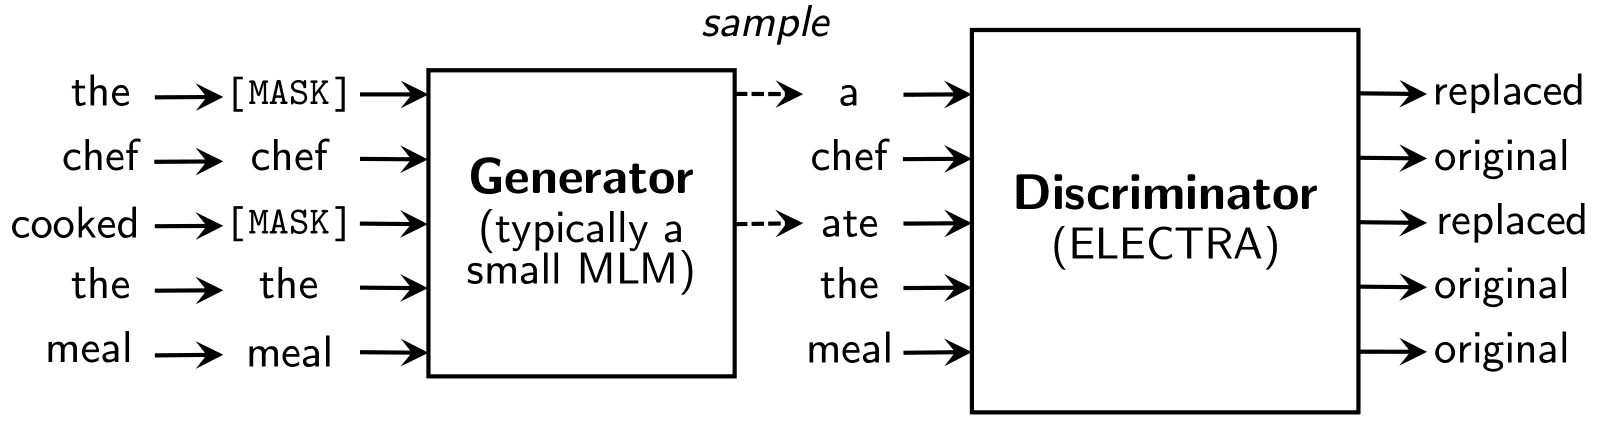
\includegraphics[width=0.85\linewidth]{electra-pretraining}
  \caption{ELECTRA RTD pre-training task (image courtesy of \cite{electra})}
  \label{fig:electra}
\end{figure}

\section{Output module}\label{sec:output-module}
The output module is composed by two fully-connected layers, used to identify the start and end token indexes of the answer in the given context. The start index classifier directly receives the output of the previous modules (e.g. in the BiDAF model that would correspond to the output of the modeling layer), while the same output vector is first passed into a single layer recurrent encoder before entering into the end index classifier. This additional RNN is used to implicitly enforce the constraint that the end index should follow the start one.

We then compute a softmax over both logits, so as to obtain a start and end index probability for each token in the context. To find the correct section of context that forms the answer, we compute the joint probability distribution (by multiplying each pair of start/end probabilities, for each token) and we take the start/end indexes corresponding to the maximum combined probability (respecting the assumption that the start index must precede the end one).

Finally, thanks to HuggingFace's tokenizers \cite{tokenizers}, we are able to simply convert start/end indexes over tokens to their corresponding values over original characters' positions.

The output layer is also responsible for the computation of the loss, which is a simple mean of cross-entropy losses of the start and end token probabilities.

\chapter{Experimental setup and results}\label{chap:experiments}
 
\section{Data handling}\label{sec:data-handling}
Given the JSON training set, we decided to parse it into a suitable tabular data structure, which turned out to be useful even for subsequent pre-processing tasks. In particular, since each context has multiple question/answer pairs and each question can have multiple answers, we allocated one row for each context/question/answer triple, thus replicating the same context and question multiple times, in order to consider it as a separate example.

Regarding the splitting strategy for the dataset, we went for a simple holdout, thus setting aside $20\%$ of the whole dataset for validation purposes. The way the validation set is built guarantees that the entire set of rows referencing to the same context is kept into the same split, thus avoiding unjustifiable boosting of results.

As an additional test, we evaluated all of our models on the official SQuAD v1.1 dev set. The main difference between this dataset and the training one is that the same question can have multiple correct answers.

Moreover, models are re-trained on the whole dataset (by merging training and validation splits), so as to simulate the cross-validation strategy. About re-training, results showed that this process only gives marginal improvements at the expense of a much more difficult way of choosing the best weights snapshots (since there are no validation metrics to observe, thus leaving only training loss available). Because of this, results reported in \ref{sec:results} do not show such training runs, but only their training/validation counterparts.  

\section{Tokenization}\label{sec:tokenization}
Tokenization has the following meaning: given a string of text, its task is to split it into sub-strings (called tokens), depending on the chosen algorithm. Different models call for different tokenization pipelines. In our case, we have two macro-categories:
\begin{enumerate}
  \item Recurrent-based models tokenizer: splits words by whitespaces and punctuations, removes accents and applies a lowercasing function to all the tokens. Moreover, questions are padded (not truncated), while contexts are truncated and padded. Taking inspiration from \cite{max-context-tokens}, the maximum number of tokens for truncating contexts was fixed to $300$
  \item Transformer-based models tokenizer: splits words using the WordPiece algorithm (introduced in \cite{wordpiece}), normalizes unicode and foreign characters, removes accents and applies a lowercasing function to all the tokens, while also merging together questions and contexts as $[CLS] q_1 q_2 \dots q_n [SEP] c_1 c_2 \dots c_m [SEP]$ (it leverages the special tokens $[CLS]$ and $[SEP]$). Moreover, the combined question/context sentence is truncated to a maximum number of tokens ($512$, as in \cite{bert}) and padded to the right
\end{enumerate}
Tokenization happens on the fly at the batch level, thus enabling us to perform dynamic padding (based on the longest sequence in a batch) and avoiding the pre-tokenization overhead.

The tokenizer is also used as some kind of pre-processor, to remove from the training dataset those rows whose contexts would not contain the relative answer, after truncation.

\section{Embeddings}\label{sec:embeddings}
In recurrent-based models, tokens are numerically encoded using the standard GloVe embeddings. In particular, we tested different types of GloVe models, with different embedding dimensions:
\begin{itemize}
  \item Wikipedia 2014 and Gigaword 5 (6B tokens, 400K vocab, uncased, 300d vectors)
  \item Twitter (2B tweets, 27B tokens, 1.2M vocab, uncased, 200d vectors)
\end{itemize}

We additionally embedded two more tokens (not present in the standard GloVe vocabulary):
\begin{enumerate}
  \item $[PAD]$: the corresponding vector, which is used to pad sequences to a fixed lenght, contains all zeros
  \item $[UNK]$: the corresponding vector, which is used to handle OOV (Out Of Vocabulary) words, is the mean of all the GloVe vectors, as reported by Pennington (one of GloVe's authors) \cite{unk}
        \begin{displayquote}I've found that just taking an average of all or a subset of the word vectors produces a good unknown vector \end{displayquote}
\end{enumerate}

In Transformer-based models, we instead rely on the wrapped language models of the HuggingFace library \cite{huggingface}, so that there is no need to manually handle token embeddings.

\section{Metrics}
Models are evaluated at the end of each epoch and metrics are computed for both the training and validation set. In our case, the validation set was mainly used to track models' performance on unseen data, in order to avoid overfitting problems.

Metrics used for evaluating the models are F1 and EM (Exact Match) and they were taken from the official SQuAD evaluation script. The F1 score ($f1=\frac{2\cdot p \cdot r}{p+r}$), defined as the harmonic mean between precision ($p=\frac{TP}{TP+FP}$) and recall ($r=\frac{TP}{TP+FN}$), is computed per question and then averaged across all questions. The EM score is instead computed as the number of questions that are answered in exact same words as the ground truth, divided by the total number of questions.

Since the same question can have multiple ground truths (specifically, in the dev set), there is the need to select just one for each question. To fulfill this requirement, only the nearest ground truth for each prediction is considered: given a prediction $p=[p_s, p_e]$, where $p_s$ is the start index of the predicted answer and $p_e$ is the corresponding end index, and a set of associated ground truths $G=\{[g_s^{(0)},g_e^{(0)}], \dots, [g_s^{(n)},g_e^{(n)}]\}$, the selected ground truth is $\min_{g\in G}\Vert p - g\Vert_2$.

Moreover, we noticed that the training set does not have multiple answers for the same question, so this "nearest answer" approach comes into play only at inference time: this is actually the desired behavior, since at training time the described technique could lead to an unstable learning process, given by the non-stationarity of the target distribution.

\section{Environment}
The main third-party libraries on which the project is based on are PyTorch \cite{pytorch}, an open source machine learning framework with automatic differentiation and eager execution, and HuggingFace \cite{huggingface}, a library to build, train and deploy state of the art NLP models.

All of the training and validation processes were executed on Google Colaboratory \cite{colab}, a platform that gives the possibility to exploit some computational resources for free. In particular, Colab allows you to select a GPU runtime, that boosts the training time of neural models and most of the times we were assigned an NVIDIA Tesla T4 GPU, with 16GB of RAM.

Training and evaluation metrics, along with model checkpoints and results, are directly logged into a W\&B project \cite{wandb}, which is openly accessible \href{https://wandb.ai/wadaboa/squad-qa}{here}.

\section{Results}\label{sec:results}
Table \ref{table:results} shows the best results obtained in the training, validation and testing phases of each model, with the hyperparameters listed in table \ref{table:hyperparameters}. In particular, by "training"/"validation" we mean metrics computed on the training/validation splits described in \ref{sec:data-handling}, while "testing" represents metrics obtained on the official SQuAD v1.1 dev set.

\begin{table}[h]
  \center
  \begin{tabular}{|c|c|c|c|c|c|c|}
    \hline
    \multirow{2}{*}{}   & \multicolumn{2}{c|}{\textbf{Training}} & \multicolumn{2}{c|}{\textbf{Validation}} & \multicolumn{2}{c|}{\textbf{Test}}                                                          \\ \cline{2-7}
                        & \textbf{F1} (\%) & \textbf{EM} (\%) & \textbf{F1} (\%) & \textbf{EM} (\%) & \textbf{F1} (\%) & \textbf{EM} (\%) \\ \hline
    \textbf{Baseline}   & $36.21$ & $21.27$ & $37.19$ & $26.47$ & $38.30$ & $27.15$ \\ \hline
    \textbf{BiDAF}      & $63.42$ & $43.27$ & $68.40$ & $55.31$ & $71.15$ & $60.09$ \\ \hline
    \textbf{BERT}       & $73.68$ & $56.14$ & $80.28$ & $67.80$ & $83.17$ & $74.17$ \\ \hline
    \textbf{DistilBERT} & $73.72$ & $55.95$ & $79.26$ & $66.97$ & $82.44$ & $73.64$ \\ \hline
    \textbf{ELECTRA}    & \textbf{76.42} & \textbf{58.89} & \textbf{84.45} & \textbf{71.83} & \textbf{88.27} & \textbf{80.60} \\ \hline
  \end{tabular}
  \caption{Best results}
  \label{table:results}
\end{table}

The hyperparameters listed in table \ref{table:hyperparameters} were mainly taken from the corresponding models' papers, in order to have a well-estabilished benchmark, even though some of them were adjusted based on available resources (e.g. the batch size).

\begin{table}[h]
  \center
  \begin{tabular}{|c|c|c|c|c|}
    \hline
                        & \textbf{Epochs} & \textbf{Batch size} & \textbf{Optimizer} & \textbf{Learning rate} \\ \hline
    \textbf{Baseline}   & $30$            & $128$               & Adam               & $1e-3$                 \\ \hline
    \textbf{BiDAF}      & $12$            & $60$                & Adadelta           & $0.5$                  \\ \hline
    \textbf{BERT}       & $3$             & $8$                 & Adam               & $5e-5$                 \\ \hline
    \textbf{DistilBERT} & $3$             & $16$                & Adam               & $5e-5$                 \\ \hline
    \textbf{ELECTRA}    & $3$             & $8$                 & Adam               & $5e-5$                 \\ \hline
  \end{tabular}
  \caption{Hyperparameters}
  \label{table:hyperparameters}
\end{table}


\chapter{Analysis of results}\label{chap:analysis-results}
For the results analysis, we focused on misclassified examples on the SQuAD v1.1 dev set. In particular, table \ref{table:errors} shows some errors (defined as those answers whose EM is zero) that are common in both of our best architectures, i.e. BiDAF and ELECTRA.

The total number of errors with BiDAF is exactly \num{4222}, while ELECTRA halves this metric to \num{2062}. Instead, the amount of common errors, i.e. the questions whose predicted answer is wrong with both models, is equal to \num{1535} (almost covering all of ELECTRA's errors).

By analyzing the common errors, we can focus on the hardest examples in the dataset. In order to categorize such misclassifications, we manually observed a random subset of $50$ elements and reported (in table \ref{table:errors}) the most frequent and interesting patterns.

\begin{longtable}{m{0.30\linewidth}|m{0.6\linewidth}}
  \textbf{Error type} & \textbf{Example} \\ \hline \endhead
  Word boundaries \newline \small{(answers that are correct but are either too specific or too generic)} & \textbf{Context}: In cases where the criminalized behavior is pure speech, civil disobedience can consist simply of engaging in the forbidden speech. An example would be WBAI's broadcasting the track "Filthy Words" from a George Carlin comedy album, which eventually led to the 1978 Supreme Court case of FCC v. Pacifica Foundation. Threatening government officials is another classic way of expressing defiance toward the government and unwillingness to stand for its policies. For example, Joseph Haas was arrested for allegedly sending an email to the Lebanon, New Hampshire city councilors stating, "Wise up or die." \newline
  \textbf{Question}: What is one criminal behavior that is hard to stop by authorities? \newline
  \textbf{Answers}: [pure speech, forbidden speech, engaging in forbidden speech] \newline
  \textbf{Predictions}: [ELECTRA] speech [BiDAF] civil disobedience can consist simply of engaging in forbidden speech \\ \hline
  Question comprehension \newline \small{(answers that clearly show one of the models was not able to fully capture the meaning of the question)} & \textbf{Context}: Although Kenya is the biggest and most advanced economy in east and central Africa, and has an affluent urban minority, it has a Human Development Index (HDI) of 0.519, ranked 145 out of 186 in the world. As of 2005, 17.7\% of Kenyans lived on less than \$1.25 a day. The important agricultural sector is one of the least developed and largely inefficient, employing 75\% of the workforce compared to less than 3\% in the food secure developed countries. Kenya is usually classified as a frontier market or occasionally an emerging market, but it is not one of the least developed countries. \newline
  \textbf{Question}: What is Kenya's HDI? \newline
  \textbf{Answers}: [0519 ranked 145 out of 186 in world, 0519] \newline
  \textbf{Predictions}: [ELECTRA] human development index [BiDAF] human development index \\ \hline
  Antonyms \newline \small{(answers for which one of the models predicted the exact opposite meaning of the correct one)} & \textbf{Context}: Luther secretly returned to Wittenberg on 6 March 1522. He wrote to the Elector: "During my absence, Satan has entered my sheepfold, and committed ravages which I cannot repair by writing, but only by my personal presence and living word." For eight days in Lent, beginning on Invocavit Sunday, 9 March, Luther preached eight sermons, which became known as the "Invocavit Sermons". In these sermons, he hammered home the primacy of core Christian values such as love, patience, charity, and freedom, and reminded the citizens to trust God's word rather than violence to bring about necessary change. \newline
  \textbf{Question}: How did Luther want people to bring about change? \newline
  \textbf{Answers}: [trust gods word, love patience charity and freedom] \newline
  \textbf{Predictions}: [ELECTRA] violence [BiDAF] reminded citizens to trust gods word rather than violence \\ \hline
  Mathematical operations \newline \small{(answers that show models' limitations in producing sound outputs when math operations are expressed in natural language)} & \textbf{Context}: In July 1888, Brown and Peck negotiated a licensing deal with George Westinghouse for Tesla's polyphase induction motor and transformer designs for \$60,000 in cash and stock and a royalty of \$2.50 per AC horsepower produced by each motor. Westinghouse also hired Tesla for one year for the large fee of \$2,000 (\$52,700 in today's dollars) per month to be a consultant at the Westinghouse Electric \& Manufacturing Company's Pittsburgh labs. \newline
  \textbf{Question}: How much did Westinghouse pay for Tesla's designs? \newline
  \textbf{Answers}: [60000 in cash and stock and royalty of 250 per ac horsepower produced by each motor, 60000 in cash and stock and royalty] \newline
  \textbf{Predictions}: [ELECTRA] 60000 [BiDAF] 60000 
  \label{table:errors}
\end{longtable}

\chapter{Discussion}\label{chap:discussion}

In this work, we addressed the problem of question answering on the SQuAD v1.1 dataset, by leveraging both recurrent-based models and Transformer-based ones. Our Baseline is outperformed by every other architecture, as expected, and models based on BERT are able to almost reach human level performance, when evaluated on the F1 score metric (for reference, that is around $90\%$). It's worth to notice that current SoTA models are all based on ensembling techniques, even though the gap with good single models is getting smaller and smaller.

We mainly worked on implementing custom recurrent-based models, such as the BiDAF network, and on giving the same output interface to each and every model, so as to gain modularity and fairness in the evaluation metrics of the backbone.

Evaluation was done on the training and validation splits of the whole dataset and on a separate test set, which is the official SQuAD v1.1 dev set: our results are on par with those reported in the literature.

Further interesting analysis could be performed on the produced outputs, to reach a better understanding of the implemented models. Anyway, conducted experiments show that both recurrent-based and Transformer-based models perform similar errors, such as those on word boundaries and question comprehension. The total number of errors, in the SQuAD v1.1 dev set, that are common in every model is exactly \num{940}.

Future improvements could be related to including character embeddings in the BiDAF architecture (as done in the original paper), using a better fine-tuning procedure for Transformer-based models (as described in \ref{chap:introduction}) and handling OOV words with more sophisticated procedures for recurrent-based models. Other things to try are the following: stacking a BiDAF architecture on top of a BERT one or simply modifying the output layer to include other modules, like convolutional ones.

\printbibliography
\end{document}
